%!TeX program = xelatex

\documentclass[aspectratio=169]{beamer}
\usepackage[english]{babel}
\usepackage{fontspec}
\usepackage{graphicx}
\usepackage{xcolor}
\usepackage{xltxtra}
\usepackage{hyperref}
\usepackage{unicode-math}
\usepackage{tcolorbox}
\tcbuselibrary{skins}
\usepackage{tikz}

\setmainfont{Iosevka NFM}
\setmonofont{Iosevka NFM}
\setsansfont{Iosevka NFM}
\setromanfont{Iosevka NFM Italic}
\setmathfont{Latin Modern Math}

\usetheme{Warsaw}
\usefonttheme{professionalfonts}
\setbeamertemplate{navigation symbols}{}
\setbeamertemplate{headline}{}
\setbeamertemplate{bibliography item}[text]

\definecolor{GreenMain}{RGB}{67,160,71}
\definecolor{GreenDark}{RGB}{27,94,32}
\definecolor{GreenAlt}{RGB}{129,199,132}

\definecolor{GreenOne}{RGB}{232,245,233}
\definecolor{GreenTwo}{RGB}{200,200,200}
\definecolor{TealThr}{RGB}{0,137,123}

\definecolor{NearBlack}{RGB}{26,71,42}
\definecolor{NearWhite}{RGB}{241,248,233}
\definecolor{AccentGold}{RGB}{255,111,97}

\setbeamercolor{structure}{fg=GreenMain}
\setbeamercolor{palette primary}{fg=white,bg=GreenDark}
\setbeamercolor{palette secondary}{fg=white,bg=GreenMain}
\setbeamercolor{palette tertiary}{fg=white,bg=GreenDark}
\setbeamercolor{palette quaternary}{fg=white,bg=GreenMain}

\setbeamercolor{title}{fg=white,bg=GreenMain}
\setbeamercolor{frametitle}{fg=white,bg=GreenMain}
\setbeamercolor{titlelike}{fg=white,bg=GreenMain}

\setbeamercolor{normal text}{fg=black,bg=white}

\setbeamercolor{block title}{fg=white,bg=GreenDark}
\setbeamercolor{block body}{fg=black,bg=GreenDark!8}

\setbeamercolor{block title alerted}{fg=white,bg=GreenMain}
\setbeamercolor{block body alerted}{fg=black,bg=GreenMain!10}

\setbeamercolor{block title example}{fg=white,bg=GreenAlt}
\setbeamercolor{block body example}{fg=black,bg=GreenOne!30}

\setbeamercolor{itemize item}{fg=GreenDark}
\setbeamercolor{itemize subitem}{fg=GreenMain}
\setbeamercolor{enumerate item}{fg=GreenDark}

\setbeamercolor{title in head/foot}{fg=white,bg=GreenDark}
\setbeamercolor{author in head/foot}{fg=white,bg=NearBlack}
\setbeamercolor{slidecnt in head/foot}{fg=white,bg=GreenTwo}

\newlength{\fttileft}
\setlength{\fttileft}{\dimexpr(\paperwidth-\textwidth)/2\relax}

\setbeamertemplate{frametitle}{%
        \nointerlineskip%
        \hbox to \textwidth{%
                \hspace*{-\fttileft}%
                
\begin{tikzpicture}[inner sep=0pt, outer sep=0pt]
                        \shade[left color=GreenDark, right color=GreenAlt]
                        (0,0) rectangle (\paperwidth,0.8);
                        \node[anchor=west, text=white, font=\large]
                        at (0.3,0.4) {\insertframetitle};
                \end{tikzpicture}%
        \hss}%
}

\setbeamertemplate{footline}{
        \leavevmode%
        \hbox{%
                \begin{beamercolorbox}[wd=.72\paperwidth,ht=2.8ex,dp=1.2ex,leftskip=1em]{title
                        in head/foot}%
                        \inserttitle
                \end{beamercolorbox}%
                \begin{beamercolorbox}[wd=.14\paperwidth,ht=2.8ex,dp=1.2ex,center]{author
                        in head/foot}%
                        \insertshortauthor
                \end{beamercolorbox}%
                \begin{beamercolorbox}[wd=.14\paperwidth,ht=2.8ex,dp=1.2ex,center]{slidecnt
                        in head/foot}%
                        \insertframenumber/\inserttotalframenumber
                \end{beamercolorbox}%
        }%
        \vskip0pt%
}

\newtcolorbox{shadowbox}{
        enhanced,
        colback=GreenOne,
        colframe=white,
        boxrule=0pt,
        sharp corners=all,
        arc=6pt,
        drop shadow,
        left=4mm,
        right=4mm,
        top=2mm,
        bottom=2mm
}

\newtcolorbox{shadowbox2}{
        enhanced,
        colback=NearWhite,
        colframe=white,
        boxrule=0pt,
        arc=4pt,
        outer arc=4pt,
        fuzzy shadow={0mm}{-1.3mm}{0mm}{0.3mm}{black!30},
        coltext=NearBlack,
        halign=center,
        fontupper=\centering,
        left=4mm,
        right=4mm,
        top=2mm,
        bottom=2mm
}

\title[Method of Exhaustion]{The Method of Exhaustion}
\subtitle{How Ancient Greek Geometry Bounded the Infinite}

\author{Pavel Shago}

\institute{
        Saint Petersburg State University\\
        \vspace{0.2cm}
        History of Mathematics in English
}

\date{\small April 24, 2026}

\begin{document}

\frame{\titlepage}

\begin{frame}{A Number That Was Not a Number}
        A Pythagorean drew the diagonal of a unit square and asked
        for its length.

        \vspace{0.3cm}
        \[
                \text{diagonal} = \sqrt{2}.
        \]

        \vspace{0.2cm}
        No ratio of integers produces it. For a school that believed
        \emph{every magnitude is a ratio of integers}, this was a
        collapse, not a curiosity.

        \vspace{0.4cm}
        \begin{shadowbox}
                And this was the \emph{easy} case. Now ask for the
                ratio of a circle's circumference to its diameter.
                Not a ratio of integers. Not a root of a polynomial.
                Not even constructible with straightedge and compass.

                \vspace{0.2cm}
                How do you prove \emph{anything} about the area of a
                circle in a geometry that forbids infinity as an object?
        \end{shadowbox}
\end{frame}

\begin{frame}{The Barrier, Stated Precisely}
        Greek geometry had two tools for comparing figures:

        \vspace{0.3cm}
        \begin{columns}
                \begin{column}{0.48\textwidth}
                        \textbf{Direct comparison}\\
                        Cut a polygon into pieces, rearrange into
                        another polygon of known area.
                \end{column}
                \begin{column}{0.48\textwidth}
                        \textbf{Similarity ratios}\\
                        Two figures of the same shape: areas in ratio
                        of squares on linear parts.
                \end{column}
        \end{columns}

        \vspace{0.5cm}
        Both are finite. Neither works for a circle, a parabolic
        segment, or a sphere.

        \vspace{0.4cm}
        Antiphon (5th c.\,BCE) proposed: inscribe polygons of
        doubling sides until they \emph{become} the circle. The
        Greeks rejected this. ``Eventually equals'' is a claim about
        infinity --- and infinity is not an object of proof.

        \vspace{0.3cm}
        \textbf{The real problem was proof-theoretic}, not numerical.
\end{frame}

\begin{frame}{Eudoxus Rebuilds the Foundation}
        Eudoxus of Cnidus ($\sim$390--337\,BCE) answered with a new
        definition of equality of ratios of magnitudes (Euclid,
        \emph{Elements}, Book V, Def.~5):

        \vspace{0.2cm}
        \begin{shadowbox}
                $a:b = c:d$ iff for all positive integers $m,n$,
                \[
                        ma > nb \iff mc > nd,
                        \qquad
                        ma = nb \iff mc = nd.
                \]
        \end{shadowbox}

        \vspace{0.2cm}
        Two ratios are equal iff they agree on \emph{every} rational
        test. The ratio is defined by its behaviour against all
        rationals --- no numerical value is ever produced.

        \vspace{0.2cm}
        \textcolor{TealThr}{\textbf{Modern echo.}} This is Dedekind's
        construction of the real numbers (1872). Eudoxus anticipated
        it by 2200 years.
\end{frame}

\begin{frame}{Controlling the Infinite With the Finite}
        One technical lemma does the heavy lifting (\emph{Elements},
        Book X, Prop.~1):

        \vspace{0.2cm}
        \begin{shadowbox}
                If from any magnitude one subtracts at least half,
                then from the remainder at least half, and so on, the
                remainder eventually becomes less than any given
                magnitude of the same kind.
        \end{shadowbox}

        \vspace{0.2cm}
        Modern restatement: for every $\varepsilon>0$ and every $M$,
        there exists $n$ with $\big(\tfrac{1}{2}\big)^{n} M < \varepsilon$.

        \vspace{0.2cm}
        The statement is \emph{finite}. It never says ``as $n \to
        \infty$.'' It says: \textbf{for every tolerance, eventually}.

        \vspace{0.2cm}
        \textcolor{TealThr}{\textbf{Modern echo.}} The
        $\varepsilon$-$\delta$ discipline of Cauchy (1821) and
        Weierstrass, 2300 years early.
\end{frame}

\begin{frame}{The Exhaustion Schema}
        To prove $\operatorname{Area}(\text{curved}) = A$:

        \begin{block}{Upper branch}
                Suppose the area exceeds $A$. Inscribe polygons,
                halving the uncovered region each step, until the
                remainder is less than (area~$-\,A$). The inscribed
                polygon then has area greater than $A$ ---
                impossible. Contradiction.
        \end{block}

        \begin{block}{Lower branch}
                Suppose the area is less than $A$. Circumscribe
                polygons; their excess shrinks below $(A -
                \text{area})$. Same contradiction, from the other side.
        \end{block}

        Therefore the area equals $A$. \textbf{No limit is ever
        taken.} The word ``infinite'' does not appear in the proof.

        \vspace{0.1cm}
        \textcolor{TealThr}{\textbf{Modern echo.}} Riemann
        integration: $\underline{S}_n \le \int f \le \overline{S}_n$,
        and the gap shrinks.
\end{frame}

\begin{frame}{Euclid Applies the Machine}
        \emph{Elements} XII.2:
        \[
                \frac{\operatorname{Area}(C_1)}{\operatorname{Area}(C_2)}
                \;=\; \frac{d_1^{\,2}}{d_2^{\,2}}.
        \]

        \vspace{0.3cm}
        Notice what this result \emph{is} and \emph{is not}:
        \begin{itemize}
                \item \textbf{It is not} a value of $\pi$. No number
                        for circle area appears.
                \item \textbf{It is} a structural law: the area of
                        any circle scales as the square of any linear dimension.
        \end{itemize}

        \vspace{0.3cm}
        Euclid proved how circles behave \emph{relative to each
        other}, without ever computing the constant that relates a
        circle to a square. The law is invariant; the constant is a
        separate, harder question.

        \vspace{0.3cm}
        \textcolor{TealThr}{\textbf{Modern echo.}} This is
        dimensional analysis: $A \sim L^2$ as a provable statement of
        geometry, not a convention of units.
\end{frame}

\begin{frame}{Archimedes Traps \texorpdfstring{$\pi$}{pi} Between Two Polygons}
        \begin{columns}
                \begin{column}{0.55\textwidth}
                        Archimedes (\emph{Measurement of a Circle},
                        $\sim$250\,BCE) applied exhaustion to a
                        96-gon --- six doublings from a hexagon:

                        \vspace{0.2cm}
                        \[
                                3 + \tfrac{10}{71} \;<\; \pi \;<\; 3
                                + \tfrac{1}{7}
                        \]
                        \[
                                3.14085\ldots \;<\; \pi \;<\; 3.14286\ldots
                        \]

                        \vspace{0.15cm}
                        Four-digit accuracy with a \emph{proven
                        enclosure}. Not a measurement --- a theorem
                        about the location of $\pi$.
                \end{column}
                \begin{column}{0.45\textwidth}
                        \centering
                        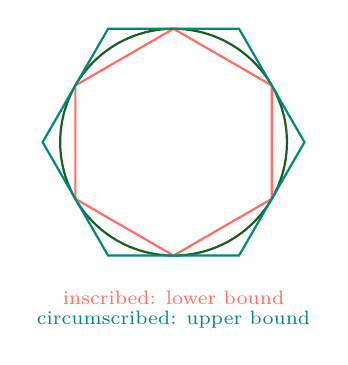
\begin{tikzpicture}[scale=0.9]
                                \def\R{1.6}
                                \pgfmathsetmacro{\Rc}{\R/cos(30)}
                                \draw[GreenDark, thick] (0,0) circle (\R);
                                \draw[AccentGold, thick]
                                (30:\R) -- (90:\R) -- (150:\R) --
                                (210:\R) -- (270:\R) -- (330:\R) -- cycle;
                                \draw[TealThr, thick]
                                (0:\Rc) -- (60:\Rc) -- (120:\Rc) --
                                (180:\Rc) -- (240:\Rc) -- (300:\Rc) -- cycle;
                                \node[text=AccentGold,
                                font=\scriptsize] at (0,-2.2)
                                {inscribed: lower bound};
                                \node[text=TealThr, font=\scriptsize]
                                at (0,-2.5) {circumscribed: upper bound};
                        \end{tikzpicture}
                \end{column}
        \end{columns}

        \vspace{0.15cm}
        \textcolor{TealThr}{\textbf{Modern echo.}} Interval
        arithmetic and verified numerics: every computed value comes
        with a proven enclosure. Archimedes' method, on hardware.
\end{frame}

\begin{frame}{What Archimedes Did Not Publish}
        Archimedes wrote a private letter to Eratosthenes ---
        \emph{The Method of Mechanical Theorems} --- lost for over
        1000 years, recovered in 1906 from a Byzantine palimpsest.

        \vspace{0.2cm}
        In it, he sliced figures into \emph{indivisibles} (infinitely
        many parallel lines) and \emph{balanced them on a lever} to
        guess areas and volumes. Mechanical intuition, not geometric proof.

        \vspace{0.2cm}
        \begin{shadowbox}
                ``It is easier to find the proof once one has
                acquired some knowledge of the questions by the
                method.'' \hfill --- Archimedes to Eratosthenes
        \end{shadowbox}

        \vspace{0.15cm}
        Archimedes used indivisibles to \textbf{discover}, then
        rewrote results as exhaustion proofs to \textbf{publish}.
        Discovery and certification separated --- the same split
        between numerical experiment and formal verification today.
\end{frame}

\begin{frame}{A Geometric Series, Without Summing Infinitely}
        \emph{Quadrature of the Parabola}: the area of a parabolic
        segment equals $\tfrac{4}{3}$ of its inscribed triangle $T$.

        \vspace{0.3cm}
        Modern view:
        \[
                T\Big(1 + \tfrac{1}{4} + \tfrac{1}{16} +
                \tfrac{1}{64} + \cdots\Big) = \tfrac{4}{3}\,T.
        \]

        \vspace{0.3cm}
        Archimedes' view: for every $n$, he filled the segment with
        triangles of total area
        \[
                T\Big(1 + \tfrac{1}{4} + \cdots + \tfrac{1}{4^{\,n}}\Big)
                \quad\text{with remainder at most}\quad
                \tfrac{1}{3}\cdot\tfrac{1}{4^{\,n}}\,T.
        \]

        \vspace{0.2cm}
        He never wrote an infinite sum. He wrote a \emph{finite
        identity} plus an \emph{error bound that can be driven below
        any magnitude}. Same answer; no appeal to infinity;
        bulletproof Greek proof.

        \vspace{0.3cm}
        \textcolor{TealThr}{\textbf{Modern echo.}} Partial sum plus
        remainder bound is still how convergence is proved.
\end{frame}

\begin{frame}{The Meta-Mathematical Mechanism}
        Three commitments of Greek mathematics made the method possible:

        \vspace{0.4cm}
        \begin{enumerate}
                \item \textbf{Magnitude over number.} Ratios of
                        geometric magnitudes, not decimal values,
                        were the primary objects. Irrationals were
                        not a problem to be solved but a type to be handled.

                        \vspace{0.15cm}
                \item \textbf{Proof over computation.} An
                        approximation without a certified error bound
                        was worthless. A bound without a computed
                        value was a theorem.

                        \vspace{0.15cm}
                \item \textbf{Finite control over infinite process.}
                        A shrinking sequence is handled by the law it
                        obeys, never by the limit point it approaches.
        \end{enumerate}

        \vspace{0.3cm}
        The method of exhaustion is these three commitments made
        procedural. Remove any one and the method collapses: it is
        inseparable from the philosophy of proof that produced it.
\end{frame}

\begin{frame}{Modern Descendants}
        The schema is the operational core of much of modern mathematics:

        \vspace{0.15cm}
        \begin{itemize}
                \item \textbf{Real numbers} (Dedekind, 1872) ---
                        direct formalisation of Eudoxus' ratios.
                \item \textbf{$\varepsilon$-$\delta$ analysis}
                        (Cauchy, Weierstrass) --- the Archimedean
                        lemma as the definition of limit.
                \item \textbf{Riemann integration} --- the curved
                        region bracketed by lower and upper sums; the
                        gap shrinks.
                \item \textbf{Interval arithmetic \& verified
                        numerics} --- Archimedes' two-sided
                        enclosure, now standard in computer-assisted proofs.
                \item \textbf{A posteriori error estimates in FEM}
                        --- approximate the solution, certify a
                        bound. Industrial scale.
        \end{itemize}

        \vspace{0.15cm}
        In every case the ancient pattern is preserved: approximate
        by simpler objects, and \emph{prove the error shrinks}.
\end{frame}

\begin{frame}{Conclusion}
        The method of exhaustion is often called ``ancient integral
        calculus.'' That label is too loose and too modest.

        \vspace{0.4cm}
        \begin{shadowbox}
                The Greek breakthrough was not a calculus algorithm.
                It was a \textbf{proof discipline for infinite
                processes that never admits infinity as an object}.
        \end{shadowbox}

        \vspace{0.4cm}
        That discipline --- approximate, bound, contradict --- is
        still the proof discipline of modern numerical analysis and
        real analysis. Greek mathematics did not find a way to
        \emph{compute} curves; it found a way to \emph{reason} about
        them. The computing came later; the reasoning is still ours.
\end{frame}

{
        \setbeamertemplate{frametitle}{}
        \begin{frame}
                \vspace*{\fill}
                \begin{center}
                        {\LARGE Thanks for your attention}
                \end{center}
                \vspace*{\fill}
        \end{frame}
}

\end{document}
